%Document the test results we did at ailab, Purdue, and Google Cloud.

\subsection{Computing resources}

Fermilab, via the LHC Physics Center (LPC), provides CPU-only batch resources and a set of interactive machines with NVIDIA Tesla T4 GPUs. Through Fermilab, we were also able to steer the allocation of cloud resources (see below) using the HepCloud~\cite{Holzman:2017jgg} framework. These resources are physically located in Illinois.
%need to be more specific?

The Google Cloud Platform (GCP) provides CPU-only virtual machines (VMs) and VMs enabled with NVIDIA Tesla T4 GPUs. By default, the CPUs are a mix of Skylake, Broadwell, Haswell, Sandy Bridge, and Ivy Bridge architectures. In GCP, we created customized machines with specified numbers of CPU threads or different ratios of CPU threads to number of GPUs. Similarly, a customized, dynamic SLURM~\cite{slurm} cluster was created that could instantiate and deplete 4-thread VMs on demand for medium-scale tests that ran jobs across $\mathcal{O}(1000)$ CPUs. The cluster's 4-thread configuration was chosen so that 4-threaded CMSSW jobs would saturate the node's resources, improving reproducibility of timing tests. CPU-only VMs could also be instantiated through HepCloud. In GCP, we also maintained GPU-enabled VMs running Triton servers that both the SLURM and HepCloud client nodes could access. These resources are physically located in Iowa.

At the Purdue CMS Tier-2 computing cluster, tests were performed with reserved CPU-only and GPU-enabled machines. The CPU-only machines are 20-core Intel E5-2660 v3 machines, and the GPU-enabled machines each have two AMD EPYC-7702 CPUs with a NVIDIA Tesla T4 GPU. Reserving these nodes allowed for controlled resource utilization, leading to more reproducible timing tests. These resources are physically located in Indiana.

It is important to note that having a diversity of locations for these resources allows for a clear demonstration of one of SONIC's key features, namely that it enables the use of non-local resources. We were able to start a server in one location and have client jobs running at another site. One such study will be presented in Section~\ref{sec:different_sites}.

\subsection{Latency Optimization}
\label{sec:algo_acceleration}
%Document the comparisons of CPU and GPU throughuts and latency of these different algorithms, maybe also with different backends, e.g., Tensorflow, ONNX, TensorRT, Pytorch, etc.

%We measure the throughputs and latency of the ParticleNet algorithm on one NVIDIA Tesla T4 GPU, with different inference backends supported in Triton: ONNX, Pytorch, and also Pytorch with TensorRT optimizations. The results are shown in Fig.~\ref{fig:throughputs_pn}.

To maximize the resource efficiency and throughput benefits of SONIC, it is necessary to start with some single-model characterization studies. For example, in order to maximize GPU usage without oversaturation, we need to find the optimal ratio of client-side CPUs to GPU, find the best batch size for inference in the Triton server, and choose the model implementation that will give the best throughput.

The latter two aspects mentioned above can be explored with the Triton Model Analyzer tool~\cite{triton_model_analyzer}. This tool feeds certain inputs in the correct tensor format to a loaded model hosted on a server, allowing for robust characterization of latency per inference or exploration of the impact of batch size.
As an example, we measure the latency and throughput of the ParticleNet (PN) algorithm for AK4 jet tagging on one NVIDIA Tesla T4 GPU, with different inference backends supported in Triton: \ONNX, \ONNX with TRT, and \PYTORCH~\cite{pytorch}. %Was this done at Purdue?
The results are shown in Fig.~\ref{fig:throughputs_pn}. 

\begin{figure}[ht]
    \centering
    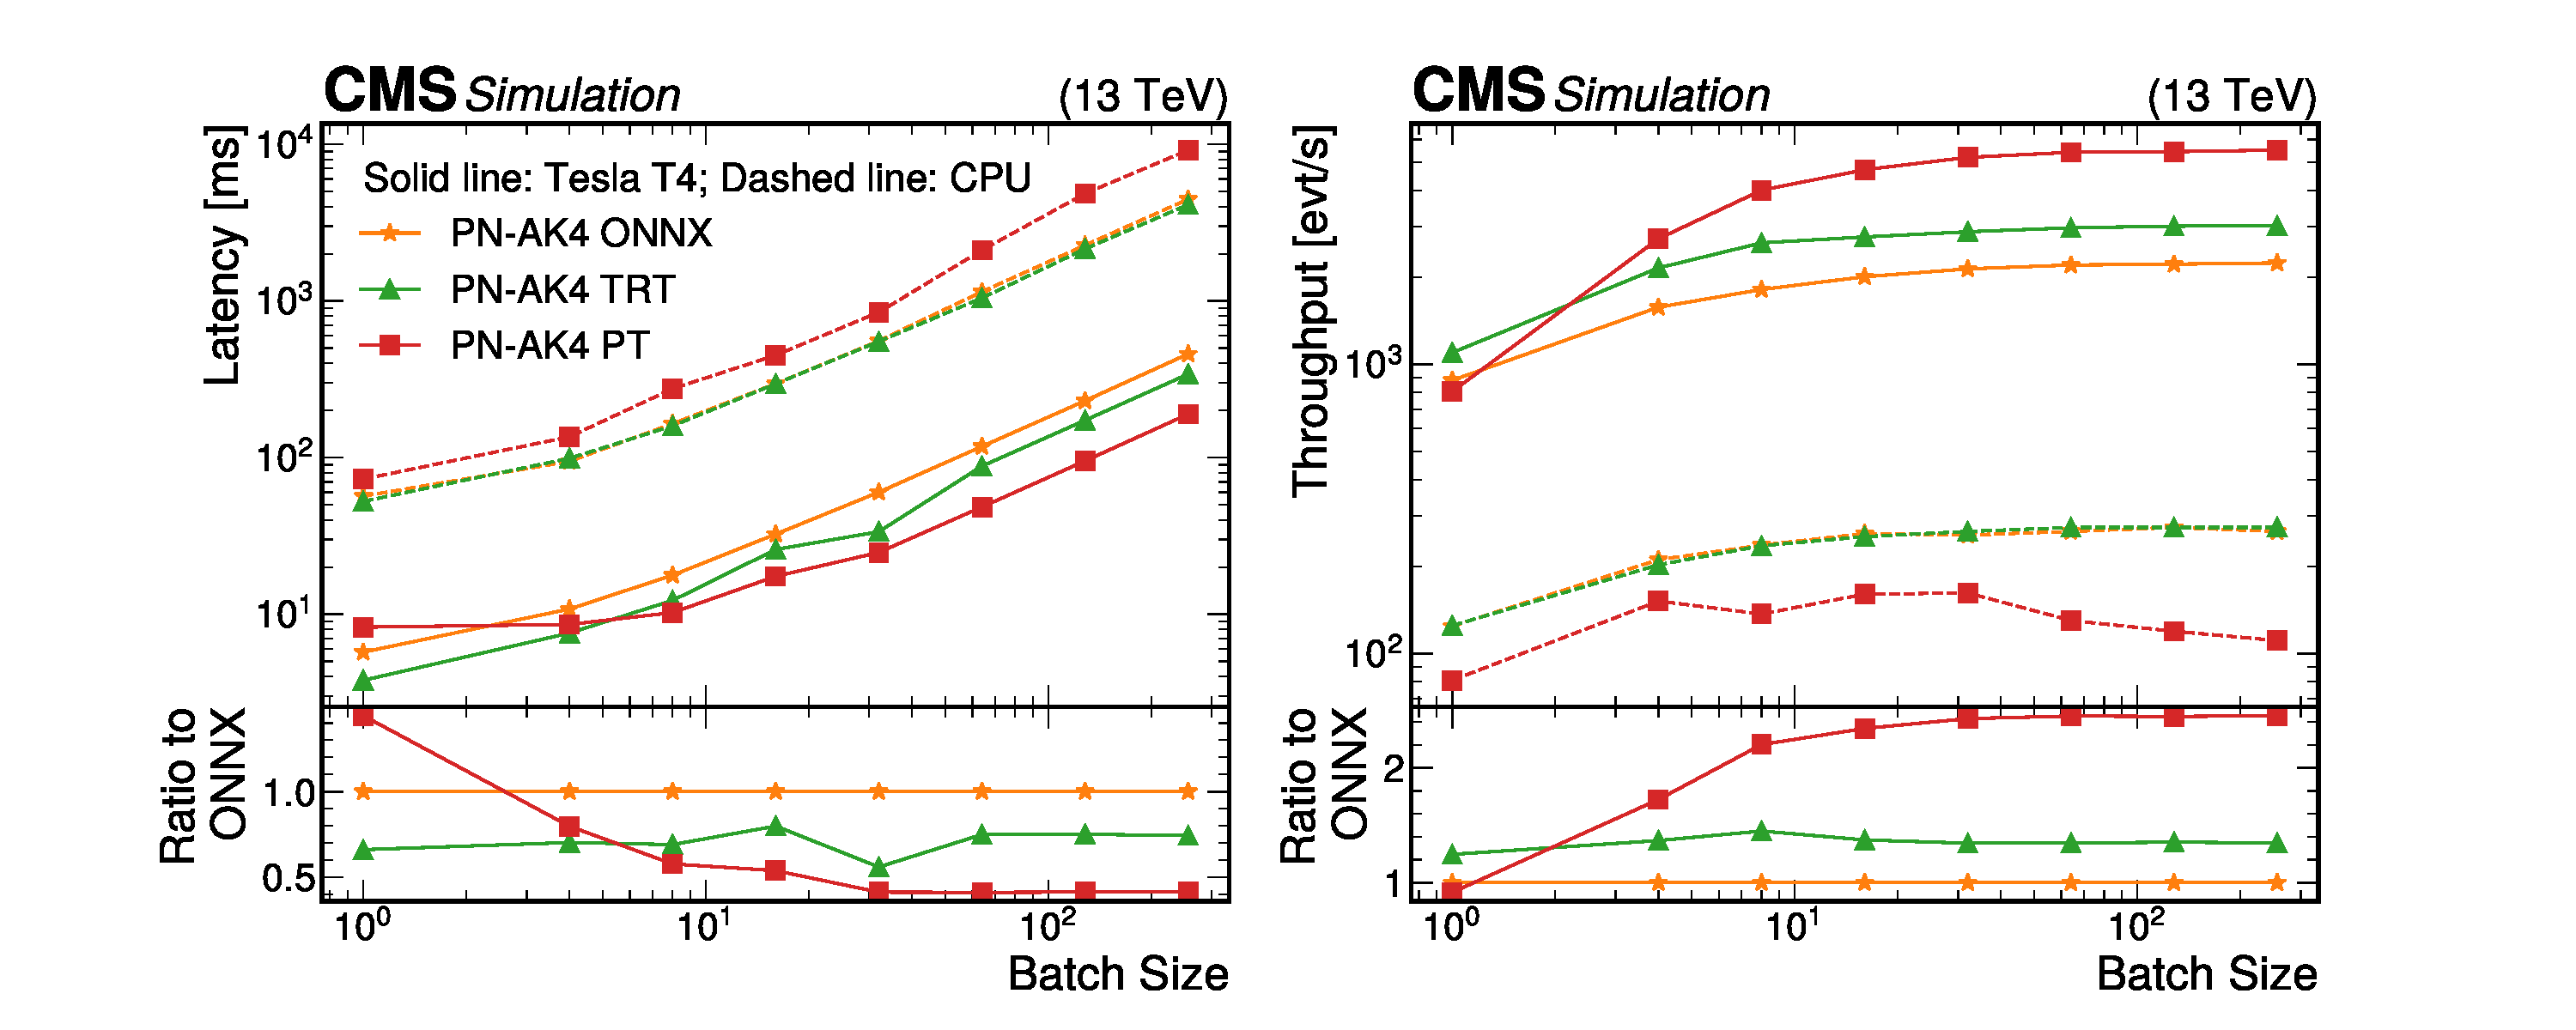
\includegraphics[width=0.98\textwidth]{plots/latencies_throughputs_pn.pdf}
    \caption{Latency (left) and throughput (right) of the AK4 ParticleNet algorithm serviced by a Triton server running on one NVIDIA Tesla T4 GPU, presented as a function of the batch size. Values are shown for different inference backends: \ONNX (orange), \ONNX with TRT (green), and \PYTORCH (red). Performance for these backends when run on a CPU-based Triton server are given in dashed lines, with the same color-to-backend correspondence.}%(\textcolor{red}{Plot will be updated; need to include some benchmarks of the throughputs and latency measured on CPUs as a function of batch size.})}
    \label{fig:throughputs_pn}
\end{figure}

For smaller batch sizes, the TRT version of PN algorithm leads to the highest throughput in total inferences per second, while at higher batch sizes, the \PYTORCH version gives higher throughput. In the SONIC-enabled version of PN in CMSSW, all of the jets in a single event are batched together, and there are typically about 16 AK4 jets per event in our \ttbar sample. To achieve higher batch sizes in a production scenario, multiple jobs would need to make an inference request from the same server within a relatively narrow time window. Triton allows us to specify a preferred batch size, such that if many inference request are queued in quick succession, the server will try to perform inferences with batches of approximately the specified size. For example, the peak throughput seems to plateau around a batch size of 100 for the PyTorch version of PN.%be achieved at a batch size of 60 for the PyTorch version of PN.
%WHICH VERSION OF PN DID WE END UP USING?  TRT?
%IN THE FIGURE, IS THAT REALLY EVENTS PER SECOND?  OR IS THAT INFERENCES PER SECOND
%What is our batching window?

The model analyzer can also approximately determine how many inferences per second a single GPU can perform before saturation. For example, for the \PYTORCH version of PN for AK4 jets, a single Tesla T4 GPU can perform about 6\,000 inferences per second without saturating. This corresponds to about 400 \textit{events} per second, given the typical number of jets per event.
Based on this, we can estimate how many CPU clients one GPU can support in parallel. A typical production configuration runs 4-threaded MiniAOD jobs, each of which processes about 3.6 events per second. Therefore, a single GPU should be able to handle about 110 4-threaded jobs in parallel running asynchronously, assuming it is being used exclusively for a single server hosting the PyTorch AK4 PN model.

This expected saturation point can be tested directly by scanning the throughput as a function of the number of CPU clients pinging one GPU server. Figure~\ref{fig:throughputs_scan_pn} shows such a test for AK4 PN, which was performed in GCP using a custom SLURM cluster. A single server running on one NVIDIA T4 GPU was started on one cloud VM, and client-side jobs were executed in VMs that had 4 CPU threads.
When offloading ParticleNet inference to GPU, we expect an improvement in the overall throughput of about 5\%, corresponding to the fraction of time taken by the total AK4 PN processing. Such an improvement is observed before saturation, where the throughput is stable as a function of the number of simultaneous CPU clients. The throughput decreases as the GPU starts to saturate, as individual client-side jobs have to wait longer for inference requests to complete and return. The throughput becomes slower than CPU-only inference at a bit after 160 parallel jobs.  This is a bit higher than the prediction from the model analyzer, likely due to the fact that the majority of the real input is padded 0s, while the model analyzer uses randomized input.
\begin{figure}[ht]
    \centering
    %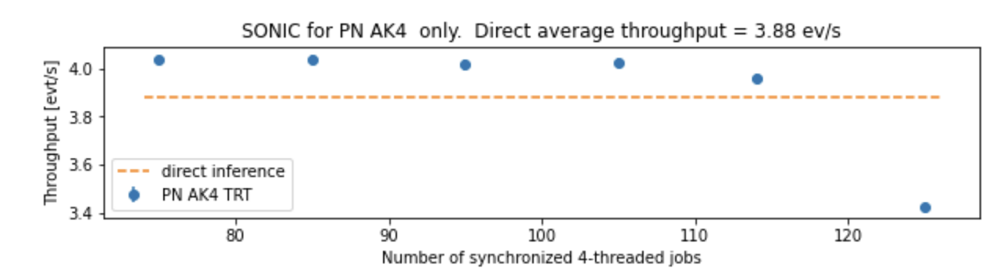
\includegraphics[width=0.90\textwidth]{plots/throughput_njobs_scan_pn.png}
    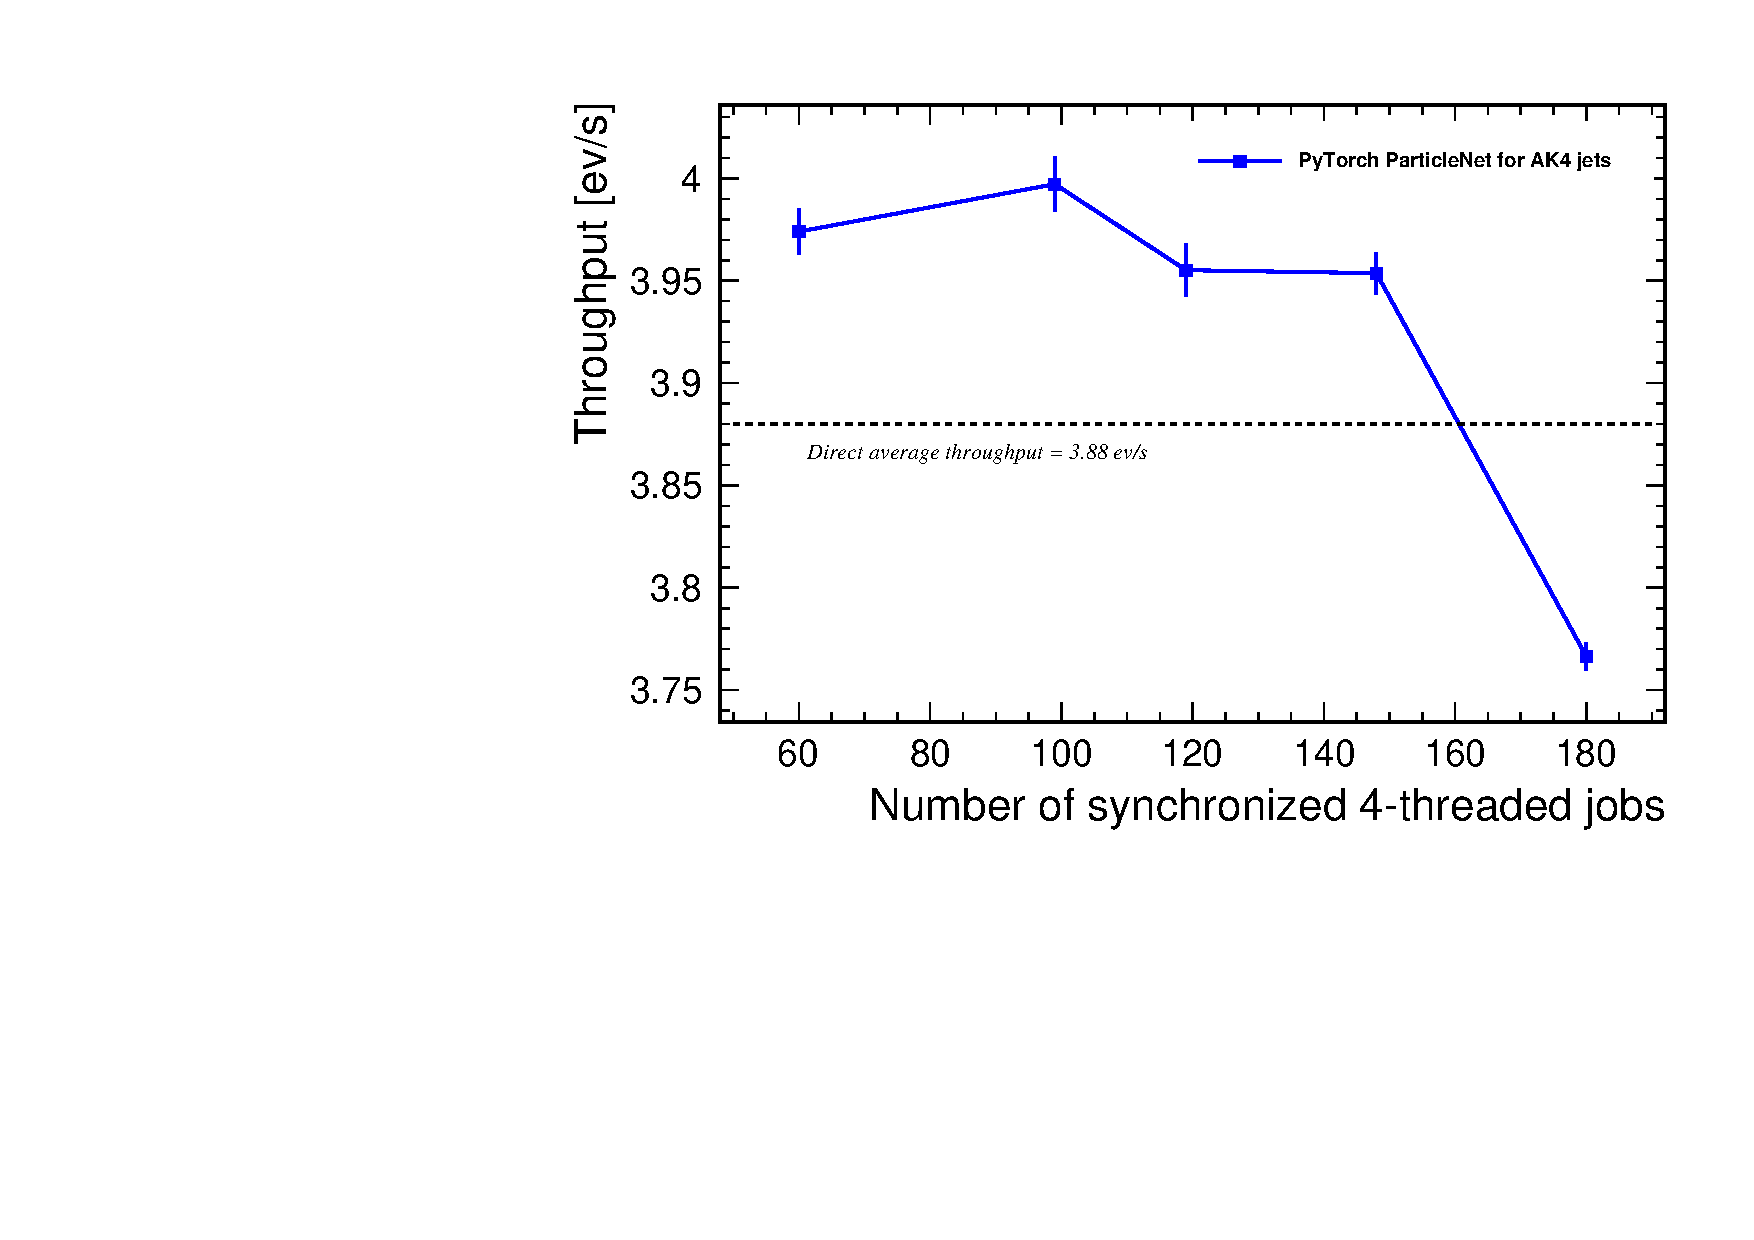
\includegraphics[width=0.70\textwidth]{plots/PN_throughput_scan_PT.pdf}
    \caption{GPU saturation scan performed in GCP, where per-event throughput is shown shown as a function of the number of parallel CPU clients for the \PYTORCH version of ParticleNet for AK4 jets. Each of the parallel jobs was run in a 4-threaded configuration.}
    \label{fig:throughputs_scan_pn}
\end{figure}

Similar analysis was performed for the other models. When all three flavors of PN for AK8 jets are hosted on a single GPU, that GPU can service about 195 simultaneous 4-threaded client jobs. For DT and DM, a single GPU hosting only one of the algorithms could service about 64 and 520 client jobs, respectively. From these saturation values, it is possible to determine the number of GPUs that would be needed to service a production job that uses a large number of client side CPUs, and it is possible to determine the ratio of the number of GPUs hosting different models. For PN and DT, the saturation points will depend on the number of jets and taus in the events in the sample being processed, such that the ratio of GPUs hosting different models and the required ratio of GPUs to CPUs is sample-dependent. As long as dynamic batching is enabled, the number of GPUs required for a model will depend roughly linearly with the number of objects per event that require an inference; for example, if a sample had half as many jets per event, it would require roughly half as many GPUs to service PN, while the number of GPUs required for DM should not change, as that model makes one inference for all events.

It should also be noted that a single GPU can host multiple models. In practice, it was found that putting only a single model on each GPU lead to about 3--5\% faster performance than putting every model on each GPU, and this split-model configuration was used in subsequent studies. However, in a scenario where samples with diverse physics content are being processing, using the every-model configuration could prove to be the easiest option, though preparatory model profiling \textit{should} still be performed to ensure that enough GPUs and model instances will be available.

\subsection{Cross-site tests}
\label{sec:different_sites}

At this point, it is worth addressing a potential bottleneck in the SONIC paradigm: increased inference latency due to physical distance between client and server and the network loads. While a previous study observed that the per-event latency difference between remote and on-premises servers is negligible~\cite{Krupa:2020bwg}, we tested this observation explicitly with the Mini-AOD workflow, with results presented in Fig.~\ref{fig:crosssites}. In this test, client-side jobs were executed at Purdue's Tier-2 computing cluster in Indiana. The blue points and lines show the throughput improvement in the Mini-AOD workflow when the client jobs communicate with Triton servers hosting all models at the same time, running on a single GPU \textit{also physically located at Purdue}. The improvement is shown as a function of the number of synchronized 4-threaded client-side jobs running at once. It can be seen that the single GPU server begins to saturate when about 10 client side jobs are sending requests at once and that the SONIC-enabled Mini-AOD workflow becomes \textit{slower} than the CPU-only workflow if more than about 17 4-threaded client-side jobs are running at once.

The green points and line in Fig.~\ref{fig:crosssites} show the throughput improvement when the client side jobs are once again run at Purdue, while the Triton server hosting all models on a single GPU is run on GCP resources, which were \textit{physically located in Iowa} for this test. Both the observed throughput increase and observed GPU saturation point are about the same for both server locations, so we can safely conclude that server location has little impact on performance, at least for client-server separations on the order of hundreds of kilometers.

%To study the possible effects of data transfers between servers and clients, we test the performances of running GPU servers on different sites. Fig~\ref{fig:crosssites} shows the test results. The CMSSW CPU clients always run at Purdue, while the servers run at Purdue and Cloud. The improvements are both around 10\% compared with directly-connected case, and the saturation point are very close. So we conclude with the current setup there is no significant impacts when running servers at different sites.

\begin{figure}[htp]
    \centering
    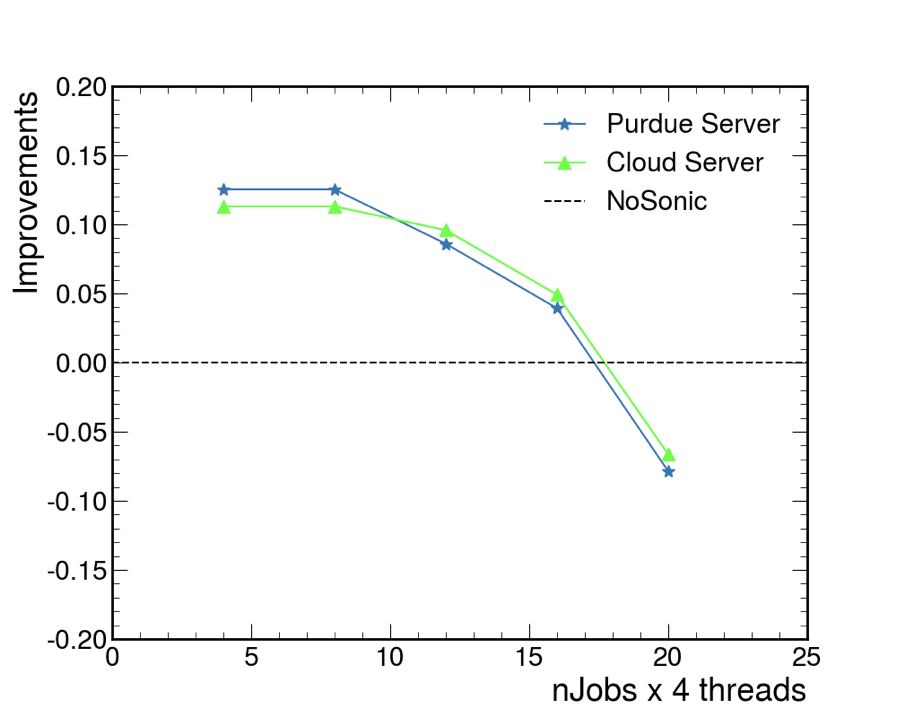
\includegraphics[width=0.60\textwidth]{plots/cloud_vs_purdue.png}
    \caption{Production tests across different sites. The CPU tasks run at Purdue, while the servers with GPU inference tasks run at Purdue (Blue) and Cloud (Green). \textcolor{red}{(Plot to be updated with better quality for publication (and better legend?).)}}
    \label{fig:crosssites}
\end{figure}

\subsection{Large-scale tests}
\label{sec:scale_out}

Finally, we run tests performed at large scale, meant to emulate realistic Mini-AOD production scenarios. This test was performed exclusively in GCP. Here, 24 NVIDIA Tesla T4 GPUs were used to host the PT version of PN for AK4 jets, 20 GPUs were used to host the PT version of all three PN models for AK8 jets, 48 GPUs were used to host DT, and 10 GPUs were used to host DM. The ratios of the number of GPUs hosting each model may not exactly match that expected from Section~\ref{sec:different_sites}; this was done because the input/output bandwidth for VMs in GCP is restricted for virtual machines with fewer CPU-cores. To maximize the allowed bandwidth, it was easiest to start up virtual machines with 4 GPUs, which is why the numbers of GPUs used for most models come in multiples of 4. For DM, two 4-GPU VMs were used along with one 2-GPU machine. Clients accessed these virtual machines via a Kubernetes load-balancer, which provided a single IP address for each model type and distributed inference requests evenly among the servers.

Client-side jobs also ran on CPU-only GCP resources, using HepCloud to dynamically allocate preemptible resources and assign jobs to the client-side VMs. Each client job was run in a 4-threaded configuration, with input data files stored locally, and each VM created in this HepCloud setup had 32 cores and 163\,840\unit{MB} of memory, meaning up to 8 simultaneous jobs could run in a single VM.

The largest test had 2\,500 synchronized client-side jobs, which amounts to 10\,000 CPU-cores. Because these jobs were run on preemptible resources, Google reserves the right to re-allocate any VM to higher priority requests from other GCP users. Of the 2\,500 job, 2\,455 completed successfully without preemption, so in the end 9\,820 client-side CPUs were used.

Preemptible resources were used to reduce the costs of running single tests. Similarly, we used a larger number of GPUs than strictly necessary to avoid the possibility that performance would \textit{not} meet the expectations from the tests described in Section~\ref{sec:algo_acceleration}, and thereby to avoid the cost of having to repeat the test potentially multiple times. For instance, based on a single-GPU saturation point of 115 4-threaded jobs, one would expect that only about 22 GPUs would be needed to service the AK4 jet PN model. So while the demonstration illustrated here uses a CPU:GPU ratio of 96:1, achieving a higher ratio is very likely possible.

The results of this large-scale test are shown in Fig.~\ref{fig:scaleout}. The SONIC-enabled jobs achieved an average throughput of 4.01 events per second, while CPU-only benchmarking jobs had a throughput of 3.55 events per second. This 12\% speed-up in throughput is about what would be expected from removing the PN, DT, and DM inference from the total MiniAOD latency.

As mentioned before, server-side VMs were optimized to allow maximal input and output bandwidth. No bottlenecks due to bandwidth were observed in this scale-out test. We noted that the maximum rate of bytes received by one of the Kubernetes load-balancers was 11.5\unit{GB/s}, which was for DT. The next-highest data input rate was 3.3\unit{GB/s} for DM, and less than 500\unit{MB/s} of input was needed for all PN models combined. The output rate was significantly smaller for each model, as most return only one or a few floating-point values as the inference result.

%discuss server-side CPU requirements?

%We perform the scale-out tests at GCP. We run around 2500 CMSSW jobs on 10K CPU cores at GCP, each job with 4 threads. The three algorithms are offloaded to around 100 NVIDIA T4 GPUs. The jobs run well with no significant issues. Fig~\ref{fig:scaleout} shows the throughput distributions of these CMSSW jobs. Compared with the directly-connected case running on CPUs (orange), we observe about 12\% throughput improvements, as expected.

\begin{figure}[htp]
    \centering
    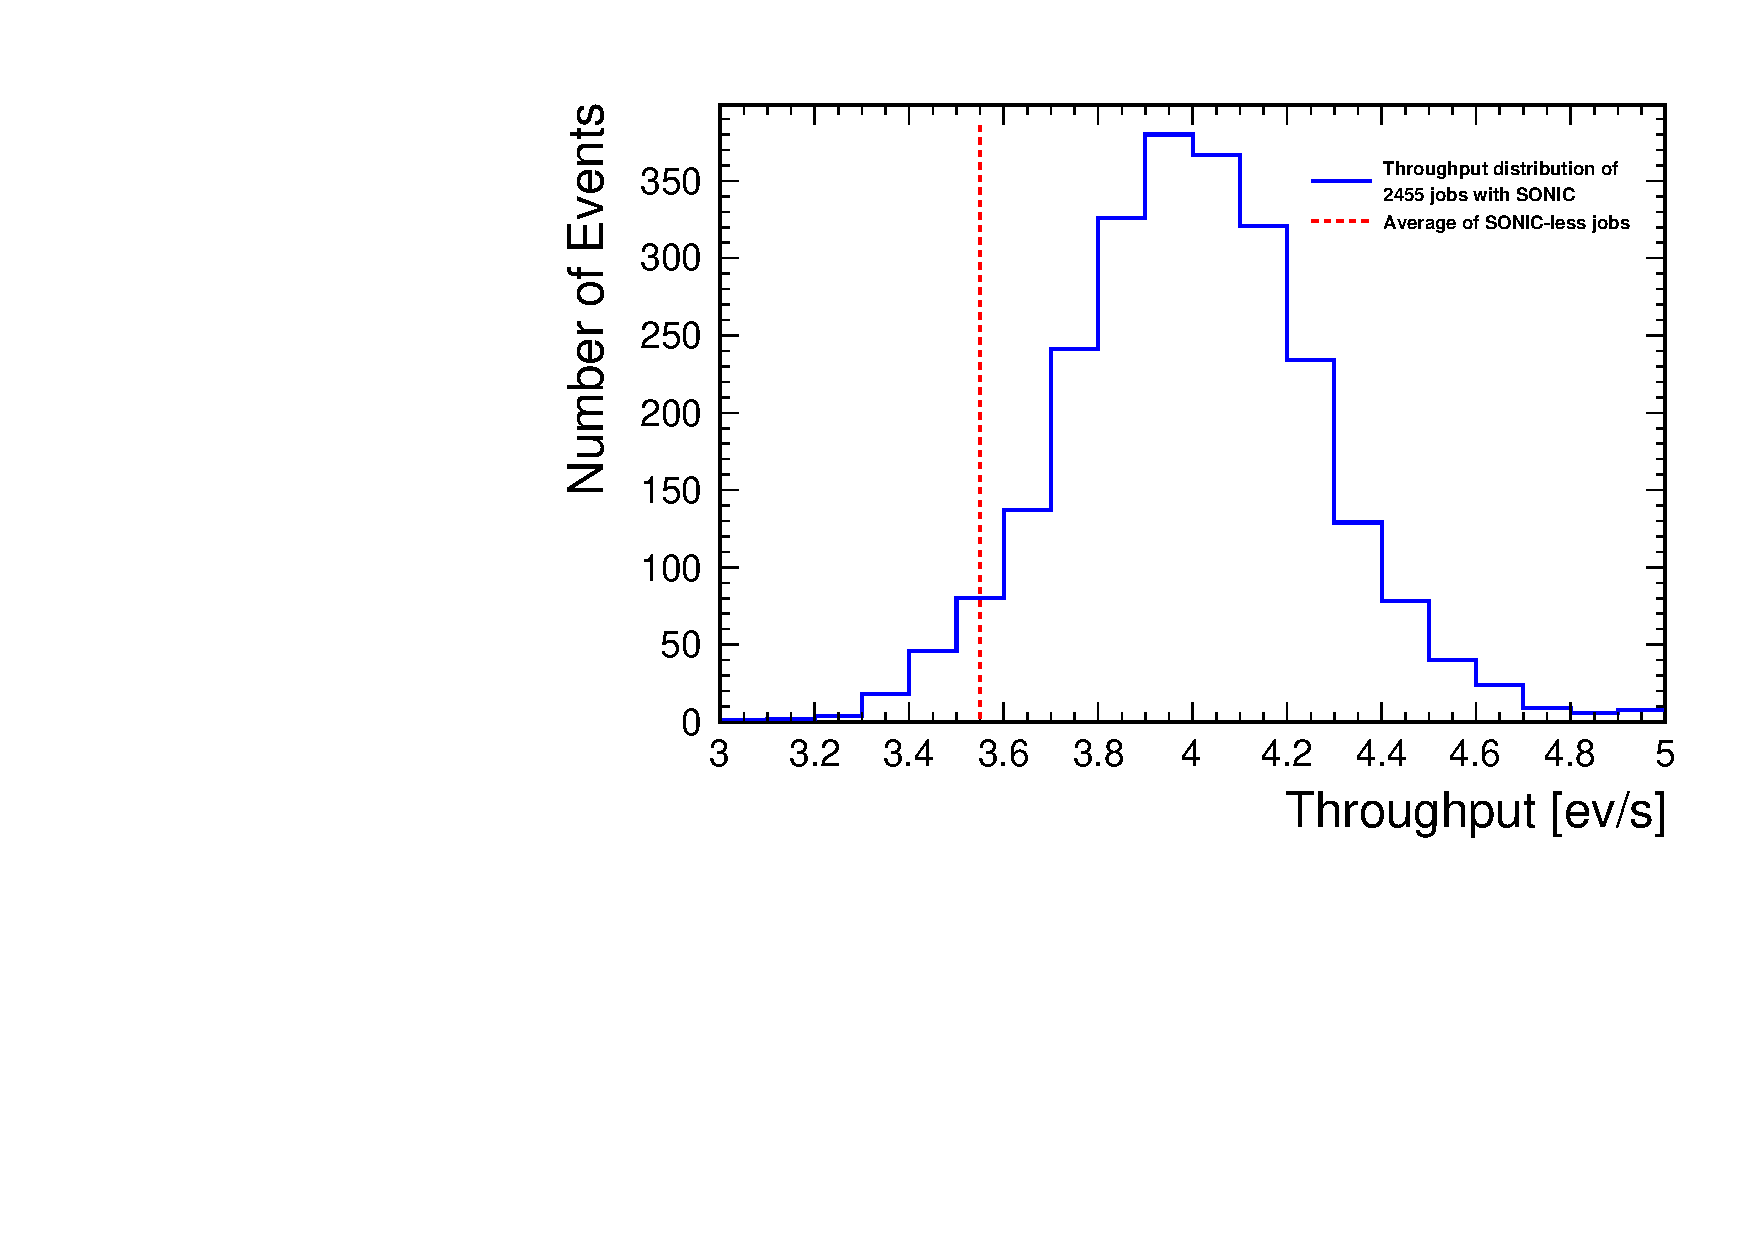
\includegraphics[width=0.70\textwidth]{plots/scale_out_test_reformat.pdf}
    \caption{Scale-out test results at Google Cloud. The average throughput of the SONIC-less workflow is 3.55\unit{ev/s}, while the average throughput of the SONIC-enabled workflow was 4.01\unit{ev/s}. The SONIC-enabled workflow thus achieves a throughput that is 12\% faster than the CPU-only version of the workflow.}
    \label{fig:scaleout}
\end{figure}

